\documentclass[conference]{IEEEtran}
\IEEEoverridecommandlockouts


%%
%% Submission ID.
%% Use this when submitting an article to a sponsored event. You'll
%% receive a unique submission ID from the organizers
%% of the event, and this ID should be used as the parameter to this command.
%%\acmSubmissionID{123-A56-BU3}
\usepackage{cite}
\usepackage{amsmath,amssymb,amsfonts}
\usepackage{algorithmic}
\usepackage{graphicx}
\usepackage{textcomp}
\usepackage{xcolor}
\usepackage{listings}
\usepackage{caption}
\usepackage{subcaption}
\usepackage{array}
\usepackage{framed}
\usepackage{tabularx}
\usepackage{booktabs}
\newcommand{\highlight}[1]{\begin{framed}%
  \noindent\emph{#1}
\end{framed}}

\definecolor{backcolor}{rgb}{0.95,0.95,0.92}
\colorlet{punct}{red!60!black}
\definecolor{delim}{RGB}{20,105,176}
\colorlet{numb}{magenta!60!black}

\lstdefinestyle{mystyle}{
  language=Python,
  basicstyle=\ttfamily\footnotesize,
  keywordstyle=\color{delim},
  stringstyle=\color{punct},
  commentstyle=\color{numb},
  breakatwhitespace=true,
  breaklines=true,
  keepspaces=true,
  showspaces=false,
  showstringspaces=false,
  showtabs=false,
  tabsize=2,
  stepnumber=1,
  numbersep=3pt,
  captionpos=b,
  numbers=left,
  numberstyle=\tiny\color{gray},
  backgroundcolor=\color{backcolor}
}
\lstset{style=mystyle}

\lstset{emph={%  
    assert%
    },emphstyle={\color{delim}}%
}%

\usepackage{graphicx}
\usepackage{caption}

\def\BibTeX{{\rm B\kern-.05em{\sc i\kern-.025em b}\kern-.08em
    T\kern-.1667em\lower.7ex\hbox{E}\kern-.125emX}}
    
%%%TRASH luis
\usepackage{pifont}
\newcommand{\luis}[1]{\textcolor{teal}{\ding{46}~\textbf{Luis:~}#1}}
%%%%%

\begin{document}

\title{Bridging the Gap Between Visual and Analytical Machine Learning
  Testing}

\author{\IEEEauthorblockN{1\textsuperscript{st} Given Name Surname}
\IEEEauthorblockA{\textit{dept. name of organization (of Aff.)} \\
\textit{name of organization (of Aff.)}\\
City, Country \\
email address or ORCID}
\and
\IEEEauthorblockN{2\textsuperscript{nd} Given Name Surname}
\IEEEauthorblockA{\textit{dept. name of organization (of Aff.)} \\
\textit{name of organization (of Aff.)}\\
City, Country \\
email address or ORCID}
\and
\IEEEauthorblockN{3\textsuperscript{rd} Given Name Surname}
\IEEEauthorblockA{\textit{dept. name of organization (of Aff.)} \\
\textit{name of organization (of Aff.)}\\
City, Country \\
email address or ORCID}
\and
\IEEEauthorblockN{4\textsuperscript{th} Given Name Surname}
\IEEEauthorblockA{\textit{dept. name of organization (of Aff.)} \\
\textit{name of organization (of Aff.)}\\
City, Country \\
email address or ORCID}
}

\maketitle

\begin{abstract}

Testing ML systems is a highly interactive process which demands a human-in-the-loop approach. In addition to writing tests for the code base, practitioners are required to analyse and interpret several visualisations using their domain expertise to validate if an ML system satisfies the required set of functional and non-functional properties. Visualisations are frequently used to qualitatively assess various parts of an ML pipeline. However, implicit knowledge gained from visualisations must be translated to explicit analytical tests that fail when there is change in any component of the ML pipeline. We conduct an empirical analysis of Jupyter notebooks to catalogue the state-of-the-art mappings between ML visualisations and assertions. We mine Github to collect Jupyter Notebooks that contain assertions written in Python. We develop a novel methodology to identify 1764 notebooks which contain an assertion below a visualisation. We manually analyse the 1.7K notebooks and identify 269 visualisation-assertion pairs that are semantically related to one another. We further investigate of the 269 visualisation-assertion pairs and identify three frequently occuring testing patterns. We perform an in-depth analysis of 34 visualisation-assertion pairs by reading and understanding the corresponding notebooks and find that the assertions often fail to capture all the information present in their visual counter-part. Our results indicate the need for automated tools that can reduce the manual effort required to verify visualisations used to test ML systems. And help ML practitioners formulate better analytical assertions.

\end{abstract}

\begin{IEEEkeywords}
  ML Testing, Visualisations, ???
\end{IEEEkeywords}

\section{Introduction}\label{sec:intro}

% TODO make sure that we use the terminology of "Testing Tasks" everywhere for RQ2
Visualisations are used throughout the ML development lifecycle to test various properties of the ML system. In the early stages of the ML development lifecycle, visualisations are extensively used to make sense of the data and verify its statistical properties. During the model development phase, visualisations are used to summarise metrics and contrast different learning algorithms and iteratively fine-tune ML models. Once the model is deployed in production, visualisations are used to continually monitor their performance and trigger a new training cycle once their performance drops below a certain threshold.

Building ML systems is highly iterative and experimental. Information gained from ML visualisations is used to make design and implementation decisions for the following steps of the ML pipeline. For instance, we may visualise the distribution of our training data and find that it is normally distributed. Based on this information, we may opt for a Linear Regression model which assumes normality in the underlying data. However, such expectations regarding the data may be violated once the ML system is deployed in production, where the data constantly changes as a reflect of the real world. Implicit expectations obtained from visualisations must therefore be translated to analytical tests that fail once our expectations regarding the ML system are no longer satisfied.

In contrast to prior work, we approach ML testing from a new perspective. We conduct an empirical analysis of computational notebooks obtained from Github, to understand the process of testing ML systems in practice. In particular, we focus on the combination of a qualitative form of testing (using visualisations) and a quantitative form of testing (using analytical assertions). The research questions along with the contributions of this paper are as follows.

\begin{description}
\item[RQ1.] How frequently are analytical tests formulated from visualisations created to test ML systems?

We mine 54K Jupyter notebooks from Github that contain an assertion written in Python. We develop an automated technique to identify 1764 notebooks with an assertion below a visualisation. We manually analyse the 1.7K notebooks and identify 269 visualisation-assertion (VA) pairs that are semantically related to each other. We plan to release this catalogue of VA pairs publicly.

\item[RQ2.] What patterns are frequently observed in VA pairs used to test ML systems?

We analyse the 269 VA pairs from RQ1, and observe three testing patterns that frequently occur in the VA pairs.

\item[RQ3.] Do the assertions capture all the information obtained from the corresponding visualisation?

We further perform an in-depth analyse of 34 VA pairs (and their corresponding notebooks). We observe that assertions often cannot capture all the information obtained from the visualisation.

\end{description}

Our observations indicate that formulating analytical assertions from visualisations is an emerging testing technique. However, the assertions found in this study often do not reflect the information obtained from their visual counter-part. This study finds the need for automated tools that can reduce the manual effort necessary to validate visualisations in ML systems. And help ML practitioners to formulate better analytical assertions from visualisations.

\section{Preliminaries}\label{sec:prelim}

This section summarises prior scientific work that has been done in ML Testing, computational notebooks and visual analytics. The section concludes with an overview of technical knowledge required for this paper.

\subsection{ML Testing}\label{sec:ml-testing}

Testing ML enabled software systems poses more challenges compared to their traditional counter part. While traditional software systems mature through change in their codebase, ML enabled systems additionally experience change in the training data and the machine learning model~\cite{sculley2015hidden,amershi2019software,sambasivan2021everyone}. With ML being adopted into safety-critical domains that can affect human lives, ensuring that ML systems are correct, robust to data perturbations and not biased by race, colour or gender is of paramount importance. Existing scientific literature on ML testing broadly focuses on two aspects. First, on functional properties such as correctness and robustness of the model towards unseen data. And second, on non-functional properties such as fairness, interpretability and privacy~\cite{zhang2020machine,mehrabi2021survey,chen2022fairness}.

To test the correctness of ML models, several improvements over existing test adequacy metrics have been proposed. Tools such as \textit{DeepExplore} and \textit{DeepGauge} propose new test adequacy metrics such as neuron coverage adapted for ML enabled software systems~\cite{pei2017deepexplore, ma2018deepgauge, gerasimou2020importance}. Formal verification methods have also been proposed that try to provide formal guarantee of robustness against adversarial examples. Such methods however are only feasible for statistical ML models and become computationally expensive for more complex models such as deep neural networks~\cite{zhu2021deepmemory, baluta2021scalable}. Several works have been conducted on generating and detecting adversarial inputs for ML models. Data augmentation techniques based on fuzzing, search based software testing and mutation testing have been proposed to generate adversarial examples that can be used during model training to improve its robustness~\cite{braiek2019deepevolution, gao2020fuzz, wang2021robot, zhang2020white}. It is however not possible to include all variations of adversarial examples into the training data. Thus, methods have been proposed to detect adversarial inputs during runtime~\cite{xiao2021self, wang2020dissector, wang2019adversarial, berend2020cats}.

In contrast to existing scientific contributions, we conduct a large-scale empirical analysis of Jupyter Notebooks to understand the process of testing ML systems in practice. Specifically, we focus on how ML practitioners use visualisations to test specific properties of ML systems. We further investigate how frequently ML practitioners formulate analytical tests based on the information gained from the visualisations.

\subsection{Computational Notebooks and Software Engineering}\label{sec:notebooks}

Computational notebooks have been ubiquitously adopted by the machine learning community for developing ML enabled systems. Although originally intended to promote reproducible software, computational notebooks are far from being reproducible due to lack of software engineering best practices such as separation of concern, testing and versioning~\cite{pimentel2019large,wang2020better,chattopadhyay2020wrong}.

\cite{psallidas2019data} provide an overview of the evolving landscape of computational notebooks by analysing six million Python notebooks, two million enterprise data science pipelines, source code and metadata from over 900 releases of 12 important data science libraries. Their findings can be used by system builders for improving data science tools and also by data science practitioners to understand the current trends in technologies they should focus on. \cite{pimentel2019large} mined 1.4 million notebooks from Github to conduct an empirical study on the coding practices in computational notebooks. Based on their analysis, the authors propose guidelines on improving reproducibility of computational notebooks. To enable future research on computational notebooks, \cite{quaranta2021kgtorrent} mine Kaggle~\footnote{https://kaggle.com} and present \textit{KGTorrent}, a public dataset consisting of approximately 2.5 million Jupyter notebooks written in Python. The dataset also contains a relational database dump of metadata regarding publicly available notebooks on Kaggle.

Studies with human subjects have been conducted to gain a deeper understanding of the challenges faced by ML practitioners when developing ML models inside notebooks. The results indicate that ML practitioners work in a highly iterative fashion, often experimenting with multiple strategies to analyse the data or produce meaningful visualisations~\cite{kandel2012enterprise, kery2018story, liu2019understanding, chattopadhyay2020wrong}. Studies have also been conducted to understand how practitioners generate, evaluate and manage alternative hypothesis, visual designs, methods, tools, algorithms and data sources to arrive at the final implementation~\cite{liu2019understanding,kandel2012enterprise}. The findings from these studies can be used as guidelines for improving existing notebook technologies or designing new ones.

To manage and prune the multiple versions of code that accumulate over time when developing in notebooks, \cite{head2019managing} propose a code gathering tool that allows practitioners to review and only keep the relevant version of code. Other tools such as \textit{WrangleDoc} and \textit{VizSmith} have also been proposed to aid ML practitioners when working within computational notebooks~\cite{yang2021subtle, bavishi2021vizsmith}.

% TODO still needs improvement
This study uses Jupyter Notebooks mined from Github. Jupyter notebooks have been widely adopted by the Data Science and ML communities to develop ML pipelines~\cite{wang2020assessing,pimentel2019large,quaranta2021kgtorrent}. Computational notebooks provide a rich source of data in the form of natural text, code and visualisations. Computational notebooks also allow ML practitioners to present the knowledge gained from the analysis in a narrative that can be shared with others~\cite{rule2018exploration}. We leverage the computational narrative present within notebooks to identify visualisations and assertions that are semantically linked to each other.

\subsection{Visualisations and Machine Learning}\label{sec:visualisations}

As ML augment software systems in safety-critical domains, emphasis has been put into explainability of ML models. ML models and the underlying data is complex and multi-dimensional. To combat the ``curse of dimensionality'', visual analytics has been widely adopted by the ML community to understand the data and the internal workings of ML models~\cite{yuan2021survey,hohman2019visual,wexler2020if}.

Prior studies have been conducted to understand how visual analytics techniques are currently being used in ML. \cite{yuan2021survey} conduct a systematic review of 259 papers and propose a taxonomy of visual analytics techniques for ML. \cite{hohman2019visual} conduct a survey of visual analytics techniques for Deep Learning Models. The findings of the study indicate that visual analytics has been widely adopted in ML for model explanation, interpretation, debugging and improvement.

Several tools have been proposed by the visual analytics research community to aid practitioners in understanding how their ML models operate. \cite{wexler2020if} propose \textit{What-If}, a visual analytics tool to explore alternative hypotheses, generate counterfactual reasoning, investigate decision boundaries of the model and how change in data affects the model predictions. To reduce the cognitive load of ML practitioners during model building phase, \cite{amershi2015modeltracker} propose \textit{ModelTracker}. Given a trained model and a sample dataset, ModelTracker presents all the information in traditional summary statistics along with the performance of the model.

\textit{ESCAPE}, \textit{GAM Coach}, \textit{Angler} and \textit{Drava} are a few other tools that have been proposed to handle specialised use-cases such as identifying systematic errors in ML models, generating counterfactual explanations for Generalised Additive Models, prioritising machine translation model improvements and relating human concepts with semantic dimensions extracted by ML models during disentangled representation learning\cite{ahn2023escape, wang2023gam, robertson2023angler, wang2023drava}.

In contrast to prior work which propose dedicated visual analytics tools, this study focuses on visualisations within computational notebooks. We focus on visualisations produced by AI practitioners using Python libraries (such as Matplotlib or Seaborn). Additional context provided by surrounding code and markdown cells are used to understand the motivation for creating the visualisation and the information gained from it.

\subsection{Internal Structure of Jupyter Notebooks}\label{sec:nbformat}

\begin{lstlisting}[caption={Top-level JSON format of Jupyter notebooks. See Listing~\ref{lst:cell-md},~\ref{lst:cell-code} and~\ref{lst:cell-output} for internal structure of various cells.}, label={lst:nbformat}]
{
  "metadata": {
    "kernel_info": {...},
    "language_info": {...},
  },
  "nbformat": 4,
  "nbformat_minor": 0,
  "cells": [ # dictionary of all cells in notebook ]
}
\end{lstlisting}
\begin{lstlisting}[caption={JSON structure of markdown cells.}, label={lst:cell-md}]
{
  "cell_type": "markdown",
  "metadata": {},
  "source": [
    "# Hello world example\n",
    "The following cell contains python code for greeting people!\n"
  ]
}
\end{lstlisting}

\begin{lstlisting}[caption={JSON structure of code cells.}, label={lst:cell-code}]
{
  "cell_type": "code",
  "metadata": {},
  "source": [
    "def greet(name):\n",
    "    print(f'Hello, {name}!')\n"
  ]
}
\end{lstlisting}

\begin{lstlisting}[caption={JSON structure of code cells with an image output.}, label={lst:cell-output}]
{
  "cell_type": "code",
  "metadata": {},
  "source": [...],
  "outputs": [
    {
      "output_type": "display_data",
      "data": {
        "image/png": "<base64-encoded-png-data>"
      }
    }
  ]
}
\end{lstlisting}

The data comprised within Jupyter Notebooks is stored in the JSON format, and thus can be parsed programmatically. Listing~\ref{lst:nbformat} shows the top-level JSON structure of Jupyter Notebooks, adopted from the official nbformat website.~\footnote{https://nbformat.readthedocs.io/en/latest/index.html}. For simplicity, only parts that are relevant for this study are shown and irrelevant parts are hidden using ellipsis.

Notebooks contain four top level keys namely \texttt{metadata}, \texttt{nbformat}, \texttt{nbformat\_minor} and \texttt{cells}. The \texttt{metadata}, \texttt{nbformat} and \texttt{nbformat\_minor} keys contain additional information regarding the notebook such as information regarding the kernel and the programming language used in the notebook. The \texttt{cells} key consists of a list of all cells within the notebook.

Listings~\ref{lst:cell-md},~\ref{lst:cell-code} and~\ref{lst:cell-output} present three examples of cells. Each cell is represented as a dictionary with the \texttt{cell\_type}, \texttt{metadata} and \texttt{source} keys. Cells can be of three types: ``markdown'', ``code'' or ``raw''. The contents of each cell can be found within the \texttt{source} key, as a list of strings. Outputs generated by a code cell are stored as a list within the \texttt{outputs} key as seen in Listing~\ref{lst:cell-output}. Static visualisations are stored as base64 encoded png images under the \texttt{outputs.data.image/png} key.

\subsection{Post-Condition Checks}\label{sec:post-cond}

\begin{table*}
\centering
\caption{Frequent examples of post-condition checks observed in this study.}
  \begin{tabular}{@{}m{0.2\textwidth} m{0.42\textwidth} m{0.28\textwidth}@{}}
\toprule
\emph{\textbf{Visualisation}}&
\emph{\textbf{Post-condition check}}&
\emph{\textbf{Rationale}}\\
\midrule
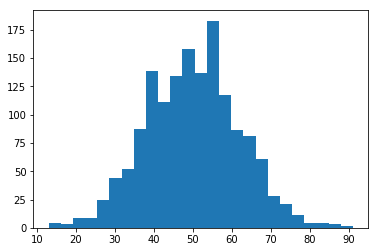
\includegraphics[width=\linewidth]{post-cond-01.png}&
\begin{lstlisting}[language=Python,belowskip=0pt,aboveskip=0pt]
assert f1.gca().has_data()
\end{lstlisting}&
The assertion checks if the output of the visualisation code cell contains an image.\\
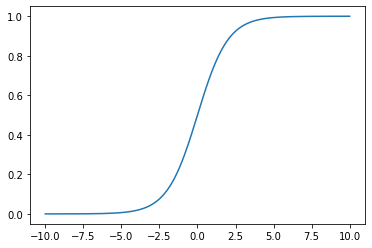
\includegraphics[width=\linewidth]{post-cond-02.png}&
\begin{lstlisting}[language=Python,belowskip=0pt,aboveskip=0pt]
assert_almost_equal(sigmoid(-50), 0, delta=1e-10)
assert_almost_equal(sigmoid(0), 0.5, delta=1e-10)
assert_almost_equal(sigmoid(50), 1, delta=1e-10)
\end{lstlisting}&
The assertions are spot-checking the sigmoid activation function.\\
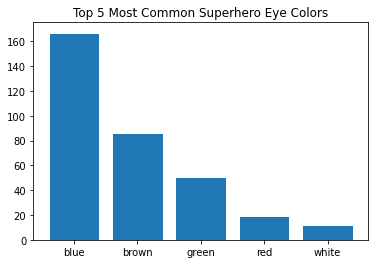
\includegraphics[width=\linewidth]{post-cond-03.png}&
\begin{lstlisting}[language=Python,belowskip=0pt,aboveskip=0pt]
# The axis should contain 5 bars
assert len(ax.containers[0]) == 5

# One of the x tick labels should be "blue"
tick_text = [tick.get_text() for tick in ax.get_xticklabels()]
assert "blue" in tick_text
\end{lstlisting}&
The asserts are validating the correctness of the visualisation itself.\\
\bottomrule
\end{tabular}
\label{tab:post-cond}
\end{table*}

We found several instances of visualisation and assertion pairs which were related to one another. However the assertions did not test a property of the ML system that was derived from the visualisation. Instead, the assertions were used to test the correctness of the code that produced the visualisation. Such assertions (and the corresponding visualisations) were excluded from this study. Table~\ref{tab:post-cond} provides examples of such post-condition checks that were frequently observed in this study.

\section{Methodology}\label{sec:method}

Figure~\ref{fig:method} summarises the methodology used to collect related VA pairs from Jupyter notebooks. The yellow boxes represent filters that were applied to the initial corpus of 54K notebooks, to obtain the final sample size of 1.7K notebooks used in the empirical study. The red boxes represent the exclusion criteria used to exclude VA pairs not relevant for this study. Text in double quotes represent the string pattern used in the search query. Each phase of the methodology is explained in more detail below.

\begin{figure*}
  \centering
  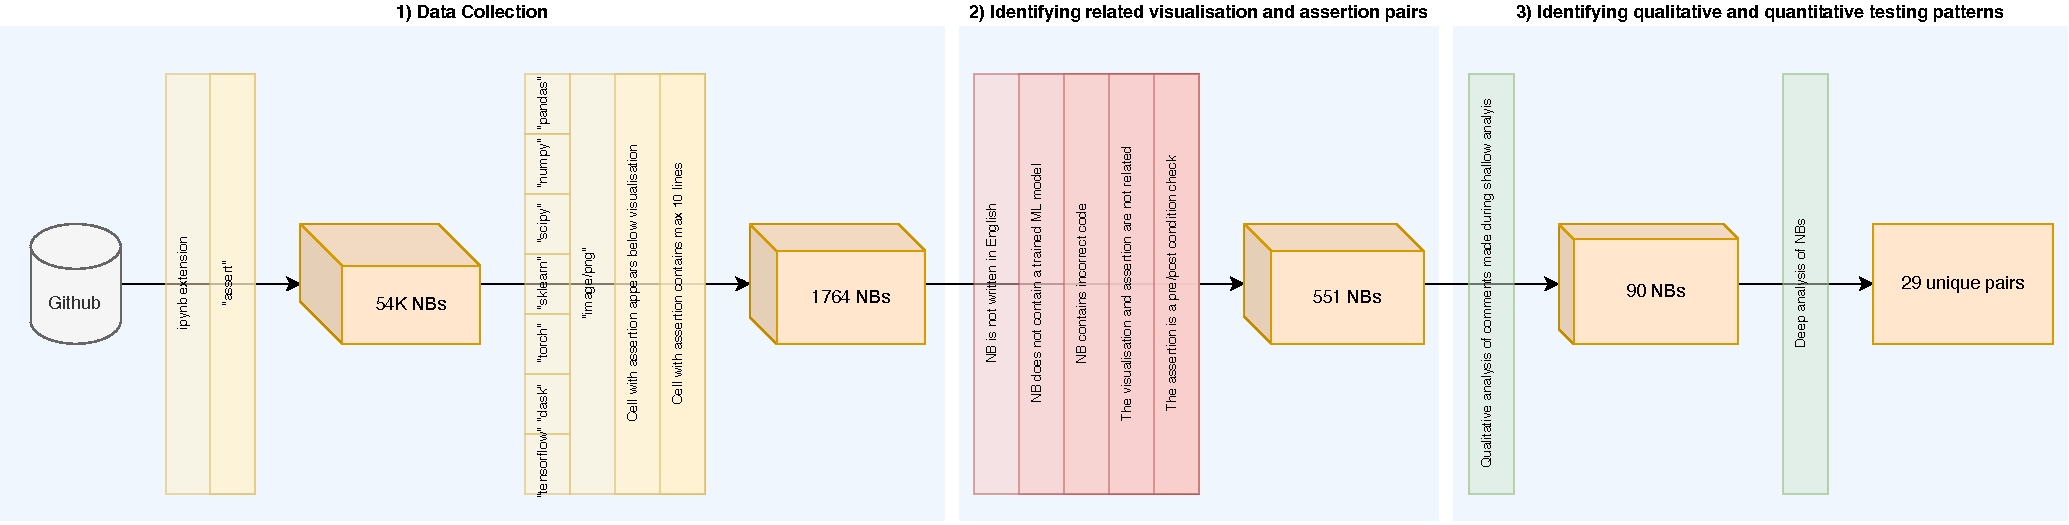
\includegraphics[width=\textwidth]{method.pdf}
  \caption{Methodology used to collect and analyse Jupyter notebooks
    in this study.}
  \label{fig:method}
\end{figure*}

\subsection{Data Collection}\label{sec:data-collect}

We mined public repositories from Github to collect $54,070$ Jupyter notebooks that contain the keyword ``assert'' in them. We use the Github advanced search syntax~\footnote{https://docs.github.com/en/search-github/searching-on-github/searching-code} to isolate Jupyter Notebook. Additionally, we include the ``assert'' keyword in the search query with an \texttt{AND} operator. The final search query is as follows: \texttt{"image/png" AND "assert" language:"Jupyter Notebook"}.\footnote{Collected on June 22, 2023}

To further reduce the sample size, we exclude notebooks that do not use popular ML or Data Science (DS) libraries. We perform a string search to identify notebooks that import at least one of the libraries. The string patterns are derived from the python module name used in the import statements. The regex search query is as follows: \texttt{tensorflow|dask|torch|sklearn|scipy|numpy| pandas}.

We programmatically parse the JSON structure of the notebooks (more details regarding the internal structure of Jupyter notebooks is presented in Section~\ref{sec:nbformat}) and represent each notebook as a pandas dataframe for further analysis. Each cell is mapped as a row in the dataframe. For each cell, we store the \texttt{cell\_type}, the \texttt{source} of the cell and the base64 encoded PNG string, into the corresponding columns of the dataframe. Notebooks without any visualisations are excluded by checking if the image column of  the dataframe is empty.

\begin{figure}
  \centering
  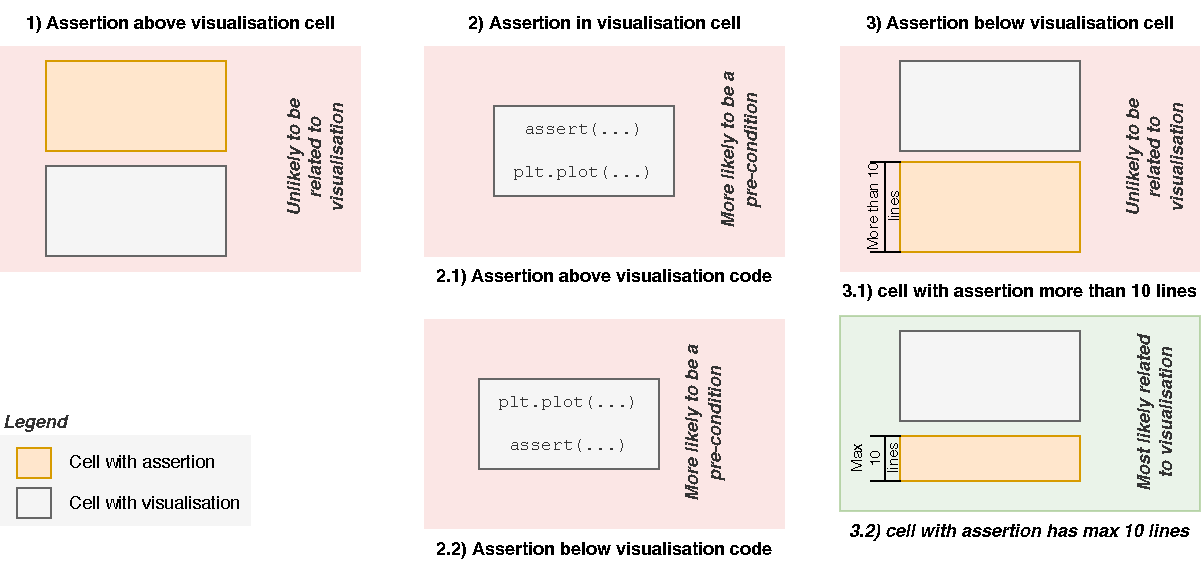
\includegraphics[width=\linewidth]{nb-structure.pdf}
  \caption{Arrangement of code cells containing assertion and
    visualisation.}\label{fig:cell-arrangement}
\end{figure}

To identify visualisation and assertion pairs that are semantically related to one another, we only consider notebooks in which the visualisation and assertion code cells appear in a specific order. Figure~\ref{fig:cell-arrangement} presents a visual representation of various arrangements of code cells that may occur in notebooks. Note that the visual representation omits markdown cells since we only consider the order of code cells in our analysis. In the actual notebook however, one or more markdown cells may be present between the visualisation and assertion cells.

We conduct the manual analysis presented in Section~\ref{sec:identify-related-pairs} for a small random sample of notebooks containing each cell arrangement. We observed the signal-to-noise ratio---notebooks with related VA pairs versus not---for each cell arrangement and picked the arrangement with the best results. Table~\ref{tab:cell-arrangement} presents the cell arrangement in ascending order of signal-to-noise ratio with a summary of our observations.

Assertions defined in a cell above the visualisation cell, were typically not related to each other. A markdown cell present between the assertion and visualisation code cells, would often mark the beginning of a new section in the notebook. In other cases, the assertions were typically checks to ensure that the visualisation code would not encounter any errors. This observation also holds for Arrangement 2.1, where the assertion is defined above the visualisation code, in the same code cell. Common examples of such checks include checking the shape of features that are used in the visualisation. Or checking that the length of the features used as the ``x''and ``y`` axes in the figure are the same to ensure a continuous line in the plot.

The signal-to-noise ratio improved in the sample of notebooks where the assertions were defined below the visualisation code. The visualisation and assertions pairs observed in Arrangement 2.2 and 3.1 were often related to each other, but were post-condition checks. Section~\ref{sec:post-cond} provides more details on post-condition checks and our rationale for excluding them from this study.

We observed the best results in notebooks with Arrangement 3.2---where the assertion cell was not longer than 10 lines and was defined below the visualisation cell. We observed that most notebook authors followed the convention of writing their motivation for the visualisation in a markdown cell, before writing the code for the visualisation. The visualisations were often followed by another markdown cell to record the author's observations. And finally, the observations were translated to a analytical test using an \texttt{assert} statement or other testing methods from external libraries. The restriction on the number of lines in the assertion cell was introduced to exclude instances where the assertion cell contained a new class definition or several helper functions that were not related to the visualisation above.

\begin{table}
  \centering
  \caption{Observations from random samples of notebooks with various
  cell arrangement.}
  \begin{tabular}{@{}l p{0.13\textwidth} p{0.27\textwidth}@{}}
    \toprule
    \emph{\textbf{ID}}&
    \emph{\textbf{Cell arrangement}} &
    \emph{\textbf{Observations}}\\
    \midrule
    1 &
    Assertion cell above visualisation cell &
    Least likely to be related to the visualisation below.\\
    \midrule
    \multicolumn{3}{l}{\textbf{Assertion and visualisation in the same code cell}}\\
    \midrule
    2.1 &
    Assertion above visualisation code &
    More likely to be a pre-condition check.\\
    2.2 &
    Assertion below visualisation code &
    More likely to be a post-condition check.\\
    \midrule
    \multicolumn{3}{l}{\textbf{Assertion cell below visualisation cell}}\\
    \midrule
    3.1 &
    Assertion cell more than 10 lines &
    Better signal-to-noise ratio compared to Arrangement 2.1. However, More likely to be post-condition check or unrelated to the visualisation above.\\
    3.2 &
    Assertion cell has max 10 lines &
    Most likely to be related to the visualisation above.\\
    \bottomrule
  \end{tabular}
  \label{tab:cell-arrangement}
\end{table}

\subsection{Identifying Related Visualisation-Assertion Pairs}\label{sec:identify-related-pairs}

The initial sample size of 54K notebooks from Github, was reduced to the final sample size of 1.7K after applying the filters presented in Section~\ref{sec:data-collect}. We analysed all 1.7K notebooks manually to further identify 269 VA pairs that were semantically related to each other.

We manually analysed the source code of the visualisation and assertion code cells. And excluded VA pairs that were not related to each other. We encountered several instances where the tracing was not straightforward due to lack of sufficient context from surrounding markdown cells or poor coding practices---such as use of obscure variable names or deeply nested function calls. In such cases, we used one-shot prompt engineering~\cite{liu2023pretrain} with the ChatGPT 4.0 model to determine if the visualisation and assertion were related to each other.

Notebooks not related to ML or Data Science (DS) were excluded from this study. We found several notebooks from other domains such as cryptography, scientific simulations, genetic algorithms and fluid dynamics. Such notebooks were captured in Phase 1 because they imported one of the popular python libraries (typically numpy or pandas). However, the visualisation and assertion pairs discovered within these notebooks were not related to ML or DS.

As explained in Section~\ref{sec:post-cond}, this study excluded assertions which did not test a property of an ML system but rather the correctness of the visualisation. Such assertions or post-condition checks were excluded from this study.

We also excluded duplicate notebooks from the study. For the purposes of this study, a notebook is labelled as a duplicate of another, when all the following conditions hold.

\begin{enumerate}
  \item Both notebooks are authored by the same author and found in the same Github repository
  \item The visualisation-assertion pairs found in the notebooks has previously been recorded in this study
  \item And the contents of the notebook is identical to a prior notebook analysed in this study
\end{enumerate}

Finally, notebooks that were not authored entirely in English or contained faulty code that did not produce a visualisation were excluded. Table~\ref{tab:exclusion-criteria} lists all exclusion criteria along with the number of notebooks that were excluded from this study.

\begin{table}
  \centering
  \caption{Inclusion-Exclusion criteria used to identify related visualisation-assertion pairs.}\label{tab:exclusion-criteria}
  \begin{tabularx}{0.47\textwidth}{@{}l X r@{}}
    \toprule
    \textbf{ID} &
    \textbf{Exclusion Criteria} &
    \textbf{\# excluded NBs}\\
    \midrule
    \textbf{EC1} &
    The visualisation and assertion are not related &
    560\\
    \textbf{EC2} &
    Notebook is not ML or DS related &
    419\\
    \textbf{EC3} &
    The assertion is a post-condition check &
    201\\
    \textbf{EC4} &
    Notebook not entirely written in English &
    164\\
    \textbf{EC5} &
    Notebook is a duplicate &
    129\\
    \textbf{EC6} &
    Notebook contains incorrect code &
    34\\
    \midrule
    \multicolumn{2}{c}{\emph{\textbf{Total number of NBs excluded:}}} &
    1507\\
    \bottomrule
  \end{tabularx}
\end{table}

\section{Results}\label{sec:result}
\subsection{RQ1: How frequently are analytical tests formulated from visualisations created to test ML systems?}\label{sec:result-rq1}

From the 1764 Jupyter notebooks that were analysed in this study, we found 269 VA pairs that were semantically related to each other.

Our observations indicate that AI practitioners formulate analytical tests based on the information gained from the visualisations that they create to test ML systems. However, this is an emerging testing practice since only 15\% of the notebooks analysed in this study exhibit this testing practice.

\subsection{RQ2: What patterns are frequently observed in VA pairs used to test ML systems?}\label{sec:result-rq2}

We further analysed the 269 VA pairs obtained from RQ1, and identified three testing patterns which are presented in Table~\ref{tab:testing-patterns} and discussed further below.

\begin{table}
  \centering
  \caption{Testing patterns observed in the visualisation-assertion pairs.}
  \begin{tabularx}{0.45\textwidth}{@{}l X r r@{}}
    \toprule
    \textbf{ID} &
    \textbf{Description} &
    \multicolumn{2}{c}{\textbf{Count}}\\
    & & Yes & No\\
    \midrule
    \textbf{P1} &
    Does the assertion use a comparison operator (such as \emph{eq, lt, gt})? &
    202 & 67\\
    \textbf{P2} &
    Does the assertion use magic thresholds? &
    101 & 168\\
    \textbf{P3} &
    Does the assertion use an external testing library (such as \texttt{numpy.testing})? &
    42 & 227\\
    \bottomrule
  \end{tabularx}
  \label{tab:testing-patterns}
\end{table}

\begin{table}
  \centering
  \caption{Most frequently occurring assertions that use a comparison operator.}
  \begin{tabular}{@{}m{0.9\linewidth}@{}}
    \toprule
    \begin{lstlisting}[language=Python,belowskip=0pt,aboveskip=0pt]
assert accuracy_score(y_test, pred) > 0.95\end{lstlisting}\\
    \begin{lstlisting}[language=Python,belowskip=0pt,aboveskip=0pt]
assert HISTORY['test_accuracy'][-1] > 0.92\end{lstlisting}\\
    \begin{lstlisting}[language=Python,belowskip=0pt,aboveskip=0pt]
assert np.mean(mean_rw_history[-10:]) > 10.
print("That's good enough for tutorial.")\end{lstlisting}\\
    \begin{lstlisting}[language=Python,belowskip=0pt,aboveskip=0pt]
assert np.mean(metrics['dev_bleu'][-10:], axis=0)[1] > 35, "We kind of need a higher bleu BLEU from you. Kind of right now."\end{lstlisting}\\
    \begin{lstlisting}[language=python,belowskip=0pt,aboveskip=0pt]
assert np.mean(dev_recall_history[-10:]) > 0.85, "Please train for at least 85% recall on test set. You may need to change vectorizer model for that."\end{lstlisting}\\
    \bottomrule
  \end{tabular}
  \label{tab:compare-op-asserts}
\end{table}

In a total of 269 VA pairs, 202 assertions (75\%) contain a comparison operator such as \emph{equal to}, \emph{lesser than} or \emph{greater than}. Table~\ref{tab:compare-op-asserts} presents the most frequently observed assertions that conform to this pattern.

An overwhelming majority of assertions compare the value of a performance metric---typically the accuracy or recall---against a ``magic threshold'' defined by the notebook author\luis{we need to absolute values here (out of 269)}. This covers 46\% of the assertions with a comparison operator. It is unclear however, how the specified thresholds were obtained since the authors do not provide additional explanation in the notebook. The threshold could have been derived based on domain expertise. Another alternative could be to define them during the Requirements Engineering phase, through discussions with all involved stakeholders\cite{CITEME}.\luis{Agathe Balayn might have something on these lines}

\begin{figure}
  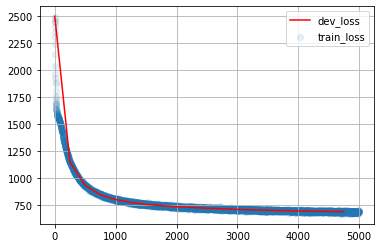
\includegraphics[width=\linewidth]{../catalogue/select-16.png}
  \caption{Visualisation of the training loss of an ML model.}\label{fig:loss}
\end{figure}

\begin{lstlisting}[language=Python, caption={Assertion to check that the mean of the first 10 observations of the loss is higher than the mean of the last 10 observations. In other words, the assertion checks if the loss function is converging to an optimal minima.}, label={lst:loss}]
assert np.mean(train_history[:10], axis=0)[1] > np.mean(train_history[-10:], axis=0)[1], "The model didn't converge."
\end{lstlisting}

In contrast to the assertions presented in Table~\ref{tab:compare-op-asserts}, Listing~\ref{lst:loss} presents an assertion that ensures that the model performs well, without using a magic threshold. The assertion checks if the mean of the first 10 observations of the loss is higher compared to the mean of the last 10 observations. In other words, the assertion ensures that the loss of the model decreased after training, and that the model was able to ``learn'' from the training set. The assertion is derived from the visualisation presented in Figure~\ref{fig:loss}, which shows the loss of the model over the training epochs.

\begin{figure}
  \subcaptionbox{Histogram showing the distribution of a feature before and after scaling.\label{fig:scale}}{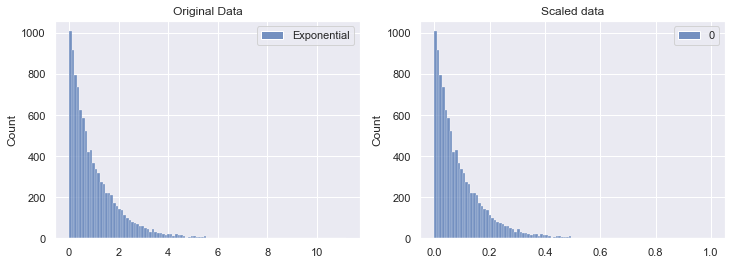
\includegraphics[width=\linewidth]{../catalogue/select-65a.png}}
  \subcaptionbox{Histogram showing the distribution of a feature before and after normalisation.\label{fig:normal}}{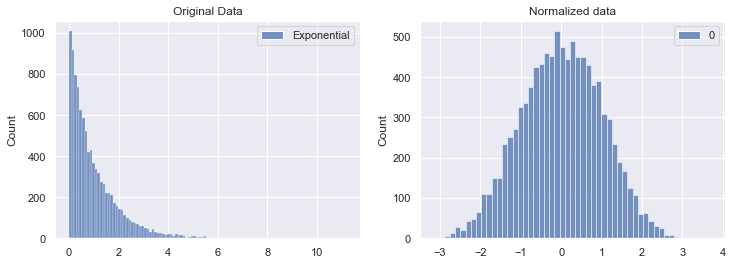
\includegraphics[width=\linewidth]{../catalogue/select-65b.png}}
  \caption{Visualisation of data before and after various data pre-processing techniques.}
  \label{fig:data-pre-process}
\end{figure}

\begin{lstlisting}[language=Python, caption={Assertion to check that the mix and max of a feature fall within specified threshold derived from the visualisation presented in Figure~\ref{fig:scale}.}, label={lst:scale}]
assert scaled_data[scaled_data.argmax()] <= 1
assert scaled_data[scaled_data.argmix()] >= 0
\end{lstlisting}

\begin{lstlisting}[language=Python, caption={Similar premise as Listing~\ref{lst:scale}, however this assertion is based on Figure~\ref{fig:normal}.}, label={lst:normal}]
assert normalized_data[normalized_data.argmax()] < 10
assert normalized_data[normalized_data.argmin()] > -7
\end{lstlisting}

Visualisations in Figure~\ref{fig:data-pre-process} were obtained from a notebook that presents a tutorial on scaling and normalization---two common data pre-processing techniques in ML. The visualisations show a comparison of the data before and after each pre-processing technique is applied to a feature from the dataset. The author performs a visual check, by comparing the distribution of the data before and after applying the pre-processing technique, using a histogram.

Listing~\ref{lst:scale} and~\ref{lst:normal} show the assertions that were defined below Figure~\ref{fig:scale} and~\ref{fig:normal} respectively. Both assertions check that the min and max of the feature is within the expected bounds after applying the respective pre-processing technique. In contrast to assertions presented in Table~\ref{tab:compare-op-asserts}, it is clear that the thresholds are derived from the corresponding visualisations.

\begin{lstlisting}[language=Python, caption={Assertion to check that an augmented image is different from the original.}, label={lst:no-comp-magic}]
assert not np.allclose(x_aug, x_original)
\end{lstlisting}

22\% of the assertions did not use a comparison operator, nor a magic threshold. Listing~\ref{lst:no-comp-magic} highlights such an assertion which is obtained from a notebook that performs image augmentation using Weighted K-Nearest Neighbours. The assertion compares the matrix representation of two images, and checks that the augmented image is different from the original.

Most notebooks examined in this study do not use any external testing libraries. 227 or 84\% of the VA pairs use the low-level Python \texttt{assert} statement to define the test directly. This aligns with our observations that majority of the assertions compare the value of a performance metric against a user defined threshold, and do not require the use of a specialised testing library. 

This study found 42 VA pairs where an external testing library was used. Listing~\ref{lst:np-almost-equal} shows an assertion that uses the \texttt{assert\_almost\_equal} method from the \texttt{numpy.testing} module. The assertion checks if the loss of the model is similar to the specified value, up to a desired precision. Due to the stochastic nature of ML, results obtained from two separate development cycles will slightly differ. The assertion presented in Listing~\ref{lst:np-almost-equal} is found to be robust towards such perturbations and will only fail if there is a significant change in the performance of the model.

\begin{lstlisting}[language=Python, caption={Assertion to check that the loss of the model is similar to the specified value.}, label={lst:np-almost-equal}]
ans4 = compute_loss(X_expanded, y, w)
np.testing.assert_almost_equal(ans4, 0.3042764) 
\end{lstlisting}

\subsection{RQ3: Does the assertion capture all the information present in the visualisation?}\label{sec:result-rq2-p3}

We performed an in-depth analysis of 34 unique VA pairs. This was conducted by reading and understanding the entire contents of the notebooks in a top-down order. During the analysis, several data points such as the primary objective of the notebook, the type of ML problem, the type of ML model and the type of data were captured. We find several instances of VA pairs where the assertion is unable to capture all the information obtained from the visualisation.

\begin{figure}
  \subcaptionbox{Visualisation of the decision boundary of a SVM with a linear kernel.\label{fig:svm-linear}}{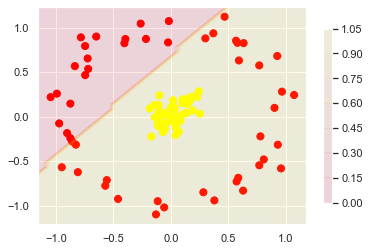
\includegraphics[width=0.49\linewidth]{../catalogue/select-04-linear.png}}
  \hfill
  \subcaptionbox{Visualisation of the decision boundary of a SVM with a RBF kernel.\label{fig:svm-rbf}}{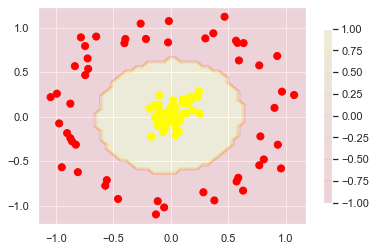
\includegraphics[width=0.49\linewidth]{../catalogue/select-04-rbf.png}}
  \caption{Visualisation of the decision boundary of a SVM trained using different kernels.}\label{fig:svm}
\end{figure}

\begin{lstlisting}[language=Python, caption={Assertion on the accuracy of the ML model.}, label={lst:svm}]
assert accuracy_score(y_test, pred) > 0.95
\end{lstlisting}

Figure~\ref{fig:svm} and Listing~\ref{lst:svm} present one such pair. Visualisations~\ref{fig:svm-linear} and~\ref{fig:svm-rbf} are obtained from a notebook that performs binary classification using Support Vector Machines (SVM). The visualisations show the two classes present in the training set, and the decision boundary of the model when trained first using a linear kernel and later with a RBF kernel.

The visualisations contain several useful information that can be used to test and debug ML models. For instance, using Visualisation~\ref{fig:svm}, ML practitioners can get a visual understanding of how well the model is able to classify the two classes in the dataset. Additionally, observing the complexity of the decision boundary is a quick way to determine if the model is under or overfitting the data. The visualisation also allows ML practitioners to compare different ML models or variants of the same ML model to iteratively find a model that best fits the underlying training data. In this case for instance, the author of the notebook first trained the SVM with a linear kernel. And upon realising that the data is not linearly separable, chose the RBF kernel.

Listing~\ref{lst:svm} shows the corresponding assertion that was defined below the visualisations. The assertion checks if the model accuracy is above a threshold specified by the author. The assertion however, is only able to capture the information pertaining to the performance of the model. While the rest of the information that is gained from the qualitative assessment using visualisation is lost.

\begin{lstlisting}[language=Python, caption={Assertion to check that the Coefficient of Determination ($R^2$) is higher than the specified threshold.}, label={lst:r2}]
r2_gru = r2_score(y_test, y_pred)
assert r2_gru > 0.6
\end{lstlisting}

\begin{figure}
  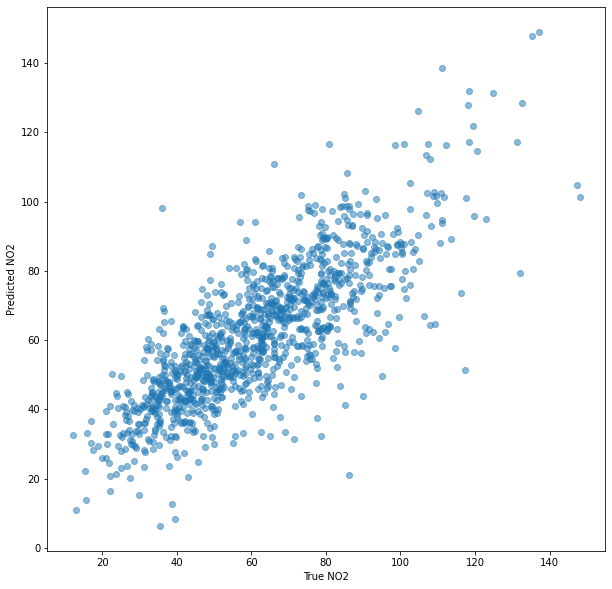
\includegraphics[width=\linewidth]{../catalogue/select-332a.png}
  \caption{Scatterplot of the actual and predicted labels of a dataset. The visualisation shows that there is a linear relationship between the true and predicted labels.}\label{fig:r2}
\end{figure}

Figure~\ref{fig:r2} shows a visualisation obtained from a notebook that trains a RNN to predict the levels of Nitrogen Dioxide ($NO_2$) in the next 24 hour window. The visualisation shows a scatterplot of the real and predicted values of $NO_2$ from the test set. A linear relationship between the ground truth and predictions is observed, indicating that the model was able to learn certain patterns from the training data. The spread of $y_{pred}$ at any given $y_{true}$ is wide. For example, at $y_{true} = 80$, the prediction can range anywhere between 30 and 120. This Indicates that the model was not able to fit the training data that well, and can be improved with fine-tuning.

Listing~\ref{lst:r2} presents the corresponding analytical test which was defined below Figure~\ref{fig:r2}. The \texttt{r2\_score} method fits a linear regression model on the true and predicted labels and computes the Coefficient of Determination ($R^2$) based on the residuals of the linear regression model. The assertion checks that the $R^2$ score of the model is always higher than $0.6$. Since the best score possible is $1.0$, the specified threshold indicates that the author wants to ensure that $y_{pred}$ and $y_{true}$ are always linearly related to each other.

Similar to Figure~\ref{fig:svm}, the visualisation in Figure~\ref{fig:r2} allows ML practitioners to visually assess if the model is under or overfitting the training data. If the spread of $y_{pred}$ is wide, it indicates that the model is under-fitting. In contrast, if the spread is very close to the diagonal line, it indicates that the model is most likely overfitting. The visualisation can also be used to verify if there are any outliers in the predictions, for a given input. The assertion in Listing~\ref{lst:r2} however, does not capture such information. It can only check if the performance of the model is better than a specific threshold.

\begin{lstlisting}[language=Python, caption={Assertion to check that each feature in a dataset is normal. The distribution of each feature is compared to that of a normal distribution using the Kolmogorov-Smirnov test for goodness of fit from the scipy library.}, label={lst:kstest}]
for feature in range(data_transformed.shape[1]):
  assert kstest(data_transformed[:, feature], 'norm').statistic < 1e-2
\end{lstlisting}

\begin{figure}
  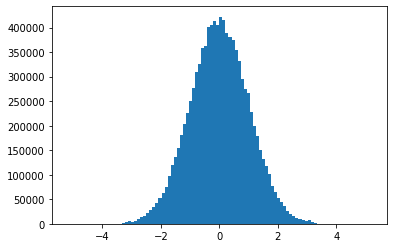
\includegraphics[width=\linewidth]{../catalogue/select-152a.png}
  \caption{Visualisation of the distribution of a feature from the dataset.}\label{fig:kstest}
\end{figure}

In contrast to Listing~\ref{lst:svm} and Listing~\ref{lst:r2}, Figure~\ref{fig:kstest} and Listing~\ref{lst:kstest} present a VA pair where the assertion captures all the information obtained from the visualisation.

The notebook author normalises the training data and performs a visual check using the visualisation presented in Figure~\ref{fig:kstest}. The visualisation shows a bell-shaped curve thus indicating that the data is normal and that the transformation was successful. The assertion in Listing~\ref{lst:kstest} formally verifies that all features in the dataset have a normal distribution. The assertion iterates through each column in the dataset and performs the Kolmogorov-Smirnov test to check that the distribution of the feature is similar to that of a normal distribution.

Checking the distribution of the training data is a very common task performed during the data understanding or exploratory data analysis phase of the ML development lifecycle. Several ML models assume normality in the underlying training data. However, in a production environment where ML models are continually trained using new batches of data, this assumption of normality may not always hold. The formal assertion presented in Listing~\ref{lst:kstest} makes this assumption explicit. And causes the automated ML pipeline to fail if our expectations regarding the data are no longer satisfied.

\section{Implications}\label{sec:discuss}

The results from RQ2 provide empirical evidence to support the use of visualisations to test various properties of ML systems.  Visualisations are an efficient and effective medium to present complex information, that is easier to interpret by humans with the aid of visual cues. Visualisations used to test ML system properties however, demand manual verification effort. Information gained from visualisations and subsequent decisions made based on this information, must be manually verified in every iteration of the ML development cycle.

% NOTE link to accumulation of technical debt due to highly experimental nature, and constant change in the system

Assertions or analytical tests extracted from ML visualisations can reduce this manual verification effort. Assertions encapsulate the knowledge gained from the visualisation with regards to the property of the ML system which is currently under test. Formal assertions document the observations made by the AI practitioner regarding the model or the data, at a specific point in time. These observations should not be violated by the future model development cycles unless the requirements of the ML system are changed. Assertions scale across organisational or personnel changes as future AI practitioners can refer to the assertions to understand how the visualisations were previously interpreted.

The results for RQ1 indicate that the combination of machine learning visualisations with analytical assertions is an emerging testing practice within the machine learning community. We found only 54,000 notebooks that contain the keyword ``assert'' and an image, while there are more than a million Jupyter notebooks available on GitHub. This suggests that the practice of assertion is still relatively uncommon.
We believe that this is due to a lack of knowledge among practitioners regarding testing approaches and the absence of adequate tooling to support the assertion of model properties. We argue that we need more guidelines on ML coding practices and that education and research of software engineering practices ought to be steered towards the specific challenges entailed from contributing to ML software.  We delve into this issue further in Section~\ref{sec:fw} \luis{I dont see this in fw and I wouldr remove this sentence because it breaks the flow of the narrative}.

Despite the efforts from some practitioners to automatically validate patterns from plots, results from RQ2 show that the classic software engineering testing practices are failing to adapt to the context of testing ML code. Very rarely assertions use dedicated API test methods. We argue that the root of this problem is two-fold: 1) the culture of testing ML code is still in its early stages and ML practitioners are not yet exploring software testing libraries, and 2) the existing testing APIs are not tuned to the specifics of ML code and practitioners have to fall back to basic built-in approaches.\luis{Side thought: we could also frame this is as: our results call for more tools that help testing ML code and that educational materials are needed to guide practitioners to testing best practices (I leave it to your judgement)}

The wide adoption of ``magic'' thresholds (\luis{add numbers from results here}) is also concerning as it can hinder to the maintainability of ML projects. While in some cases there these thresholds come a results of domain expertise and experience acquired while working in a give project, we argue that such thresholds need to be properly documented. Our results show that there is a need to help practitioners keeping these decisions documented. This could be automated using a tool to flag undocumented decisions or that would suggest boilerplate documentation in Markdown or code annotations.

Additionally, in the results from RQ2\luis{this is RQ3}, we see several examples of assertions that fail to capture all the information gained from its visual counter-part. We argue that this can lead to a mismatch of expectations in future versions of the ML software: for example, another collaborator of the project might run the code with a new version of the dataset or a different learning technique and assume that if the assertions run successfully, the expected patterns from the visualisation are also being met. After delving into some examples, we also observe that deriving assertions from validations is far from trivial: basic visualisation patterns require complex mathematical techniques that might be out of the expertise of the ML developer. We ought to bridge the gap between qualitative assessment of ML systems using visualisations and deriving analytical assertions from the visualisations. In other words, there is a need for automated tools that make this translation process easier for AI practitioners. In sum, our results showcase a gap in the current state of the art in software testing: it is failing to address the idiosyncrasies of ML code.

\section{Threats to Validity and Future Work}\label{sec:threats}

The empirical analysis presented in this study uses Jupyter notebooks mined from Github. To the best of our knowledge, \cite{pimentel2019large} and \cite{quaranta2021kgtorrent} are the only two prior studies which provide a public dataset of Jupyter Notebooks. We faced several technical challenges while trying to access the notebooks provided by these authors and thus decided to mine our own data from Github. We invite the scientific community to extend our catalogue of visual and analytical testing patterns, using the corpus of notebooks provided by the above authors.

In Section~\ref{sec:data-collect}, we intentionally keep the search criteria on Github broad by only checking for the appropriate filetype and the presence of the ``assert'' keyword. Besides being used to define tests in the Python programming language, ``assert'' also appears in several external python libraries that provide a testing interface (for instance nose, unittest and numpy). Our approach provides captures a rich variety of assertion statements while preventing the need to craft a custom search query based on an enhaustive list of keywords that appear in all Python testing libraries.

% TODO don't mention quantity of random sample; then we need to explain/defend this choice
We used an iterative approach to determine the effectiveness of each filter that was used. We applied each filter in the same order as presented in Table~\ref{tab:filters}, starting with F1. We randomly sampled 50 notebooks from the population of notebooks obtained after applying the filter. We then conduct the qualitative assessment presented in Section~\ref{REFME} and observe the number of related visualisation and assertion pairs. In each new iteration, we progressively add the other filters and include the filter if the number of relevant visualisation and assertion pairs increases.

% TODO defend use of one-shot prompt engineering for identifying related visualisation and assertion code cells; how did we mitigate this threat?

\section{Conclusion}\label{sec:conclude}


In this study, we delved into the fusion of visualizations and analytical assertions in the testing of machine learning (ML) systems. Our investigation unveiled the emerging practice of crafting analytical assertions based on visual insights, a technique that bridges the qualitative and quantitative aspects of ML testing.

Testing ML systems in Jupyter Notebooks remains a burgeoning practice, with only a minority of notebooks adopting this approach. In total, we identified 269 pairs of visualizations and assertions that exhibited semantic correlation within 1.7k notebooks. Within these pairs, our analysis unveiled several key insights: nearly 40\% of the pairs included magic thresholds, 75\% of the assertions employed comparison operators, and 16\% of the assertions made use of external testing libraries. Furthermore, we observed that 22\% of the assertions did not utilize a comparison operator or a magic threshold.

Additionally, our study brought to light recurring testing patterns, underscoring the need yo enhance the alignment between visualizations and their corresponding assertions.
This research serves as a first step in comprehending the landscape of ML testing in Notebooks, emphasizing the potential for the development of more effective tools and practices to streamline the validation of visualizations and elevate the quality of analytical assertions.

\section{Future Work}\label{sec:fw}

This study underscores the imperative to enhance the current state of machine learning (ML) testing. Our observations have pointed to several potential future directions that could advance this field:

1. Tailored Assertion Tools: There is a clear need for assertion tools specifically designed to cater to the requirements of ML practitioners. These tools should provide assistance in identifying the most suitable visualizations for testing specific properties of ML systems. Customized solutions that streamline the process of connecting visual insights to analytical assertions would significantly benefit practitioners in this domain.

2. Automation of Assertions: The manual translation of insights derived from visualizations into analytical assertions presents a substantial challenge. Future work should focus on the development of automated tools that can assist AI practitioners in this translation process. By automating the generation of assertions from visual information, these tools can promote broader adoption of assertions in ML notebooks, reducing the burden of manual effort.

3. Dynamic Testing in Real-World Scenarios: Extending ML testing to dynamic real-world scenarios is a critical avenue for future exploration. This entails developing techniques and frameworks that allow assertions to adapt to evolving data distributions, changing model requirements, and continuous system updates. Research in this area will contribute to the development of ML systems that remain reliable and relevant throughout their operational lifecycles.


\bibliographystyle{IEEEtran}
\bibliography{bibliography}

\end{document}
\endinput

